\section{\review{Beam Instrumentation}}


% ============================================
%          Beam Position Monitors
% ============================================
\subsection{\review{Beam Position Monitors}}

Beam Position Monitors (BPMs) are one of the most utilized and essential elements of beam 
diagnostics in particle accelerators. In the LHC, most of the BPMs are dual plane, and thus composed
of four electrodes, distributed as two per plane. The BPM system consists of over than 550 BPMs pear
beam, positioned along the ring, in the arcs and the IPs. The most common type, the
\textit{curved-button}, shown in \cref{fig:beam_instrumentation_bpm_button}, is typically placed
near quadrupoles~\cite{wendt_bpm_2020}.

\begin{figure}[!htb]
    \centering
    \begin{subfigure}[b]{0.45\textwidth}
        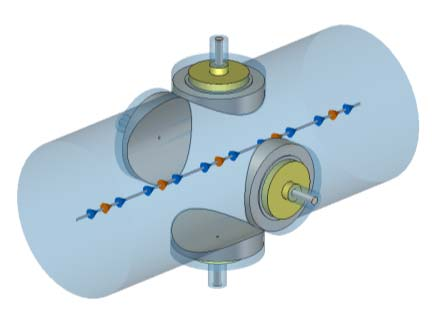
\includegraphics[width=\textwidth]{images/lhc_bpm_button.jpg}
        \caption{Button \textit{"BPM"} type BPM of the LHC~\cite{wendt_bpm_2020}.}
        \label{fig:beam_instrumentation_bpm_button}
    \end{subfigure}
    \hfill
    \begin{subfigure}[b]{0.45\textwidth}
        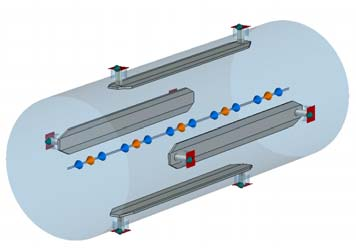
\includegraphics[width=\textwidth]{images/lhc_bpm_stripline.jpg}
        \caption{Stripline \textit{"BPMSW"} type BPM of the LHC~\cite{wendt_bpm_2020}.}
        \label{fig:beam_instrumentation_bpm_stripline}
    \end{subfigure}
\end{figure}

Other pickups such as the \textit{stripline}, shown in
\cref{fig:beam_instrumentation_bpm_stripline}, albeit more complex and expensive, offer a better
signal to noise ratio and are capable of identifying the direction of the
beam~\cite{wendt_bpm_2020}. Such features are essential for the LHC, were both beams travel through
the same aperture at the IPs.\\ 
%The BPM response is not linear with the beam position, which requires a post-processing not
%systematically implemented in accelerators beam diagnostics systems. LHC's BPMs have been simulated
%and polynomials fitted to minimize this response error~\cite{a_nosych_geometrical_2014}.


 
% ============================================
%                Collimators
% ============================================
\FloatBarrier
\subsection{\review{Collimators}}

Collimators are a crucial part of the LHC. Their purpose is to protect the machine against beam
losses and clean the outer parts of the beam~\cite{redaelli_lhc_2011}. The energy of the beams in
the LHC is high enough to not only quench the magnets, but to also damage the elements. At
injection energy, with a low intensity pilot bunch, the consequences of a loss are less severe.

%During Run 3, in 2022, a new collimator sequence was introduced, making a safe exploitation
%of the machine possible with more retracted collimators. This made measurements with higher kick
%amplitudes and larger orbit offsets, and thus momentum offsets, possible.


% ============================================
%             Beam Loss Monitors
% ============================================
\subsection{\review{Beam Loss Monitors}}

Beam Loss Monitors are detectors mounted on various elements of the accelerator, such as magnets or
collimators, to detect abnormal losses of particles. They play a crucial role in the protection of
the machine, triggering a dump when losses exceed the threshold set for their respective element. 
BLMs use ionization chambers, working on the same principle as simple Geiger counters: a tube filled
with gas, in presence of a high voltage~\cite{schmidt_machine_2014}. A picture of BLMs mounted on
the LHC is given in \cref{fig:beam_instrumentation:blm1}.

Dashboards in the control room are regularly used to monitor the losses along the ring when
performing optics measurements, as those prove to often be destructive. An example of such a
dashboard is given in \cref{fig:beam_instrumentation:blm2}.

\begin{figure}[H]
    \centering
    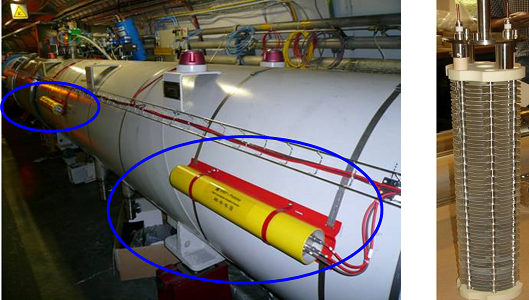
\includegraphics[width=0.6\textwidth]{images/blm.png}
    \caption{Beam Loss Monitors (BLM), in yellow, on the LHC~\cite{schmidt_machine_2014}.}
    \label{fig:beam_instrumentation:blm1}
\end{figure}

\begin{figure}[H]
    \centering
    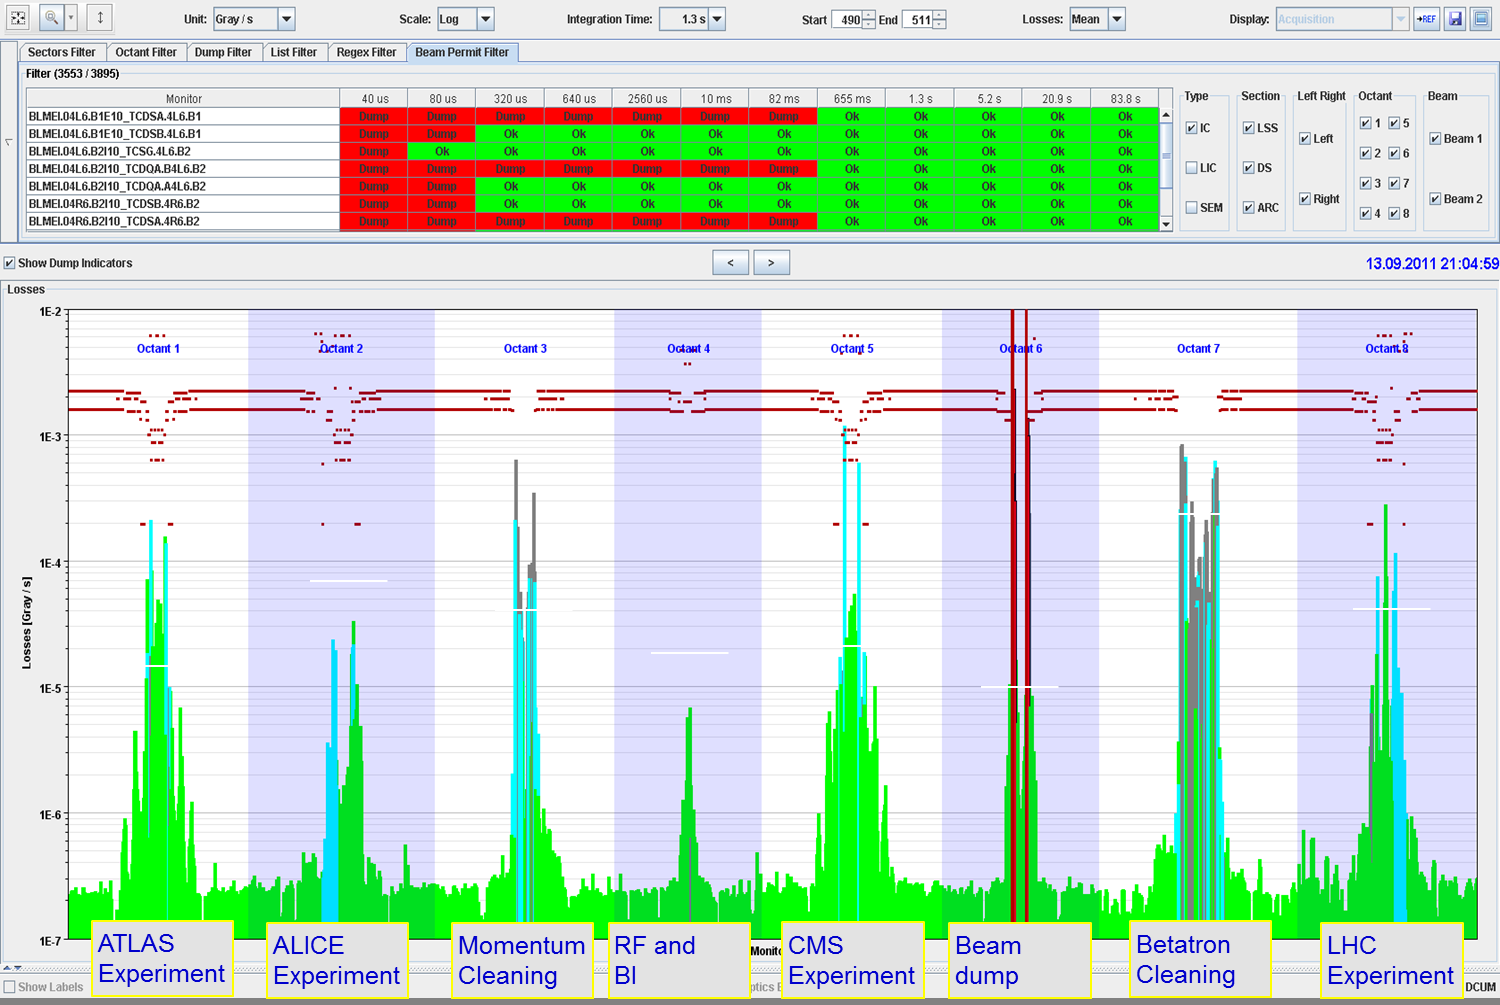
\includegraphics[width=0.6\textwidth]{images/blm2.png}
    \caption{Graphical interface used in the CERN Control Center (CCC) for instantaneous losses in
    the LHC~\cite{schmidt_machine_2014}. Different parts of the accelerator have varying dump
    thresholds.}
    \label{fig:beam_instrumentation:blm2}
\end{figure}


% ============================================
%                   BCT
% ============================================
\subsection{\review{Beam Current Transformer}}

The Beam Current Transformer (BCT) is a device used to measure the intensity of a particle beam by
detecting the current induced by the moving charge of the beam as it passes through the coil of the
BCT. The beam effectively acts as a primary coil and induces a current in the secondary coil of the
transformer.
The BCTs are designed to be able to measure intensities from pilots bunches of 8µA to total beams of
more than 860mA~\cite{odier_dcct_2009}. During optics measurements, beam intensity is often closely
monitored to ensure data quality, as certain observables may not be detectable at low intensities.

% ============================================
%                   BBQ
% ============================================
\subsection{\review{BBQ System}}

The Base-Band Tune (BBQ) system in the LHC is designed to measure the beam's tune via its
turn-by-turn signal. It operates by detecting and analyzing the signals of diode
peak-detectors~\cite{boccardi_first_2009,gasior_high_2005}. The system further implements processing
hardware and software, transmitting the acquired data to the control and logging systems.  The
system can operate with no explicit excitation, relying on the residual beam oscillations, or by
using tune kickers or frequency sweeps~\cite{boccardi_first_2009}.


% ============================================
%                 AC-Dipole
% ============================================
\subsection{\review{AC-Dipole}}

The AC dipole of the LHC is a crucial component for optics studies. Its primary function is to
excite the beam into large coherent oscillation, achieved by applying a sinusoidally oscillating
dipole field~\cite{miyamoto_parametrization_2008}. By ramping up and down adiabatically the
amplitude, large coherent oscillations can be produced without any decoherence or emittance growth.
\Cref{fig:ac_dipole} shows an example of a simulation made with an AC-Dipole. Exciting the beam to
large amplitudes make the study of linear optics, such as beta-beating easier, and that of non
linear optics such as resonances possible.

\begin{figure}
    \center
    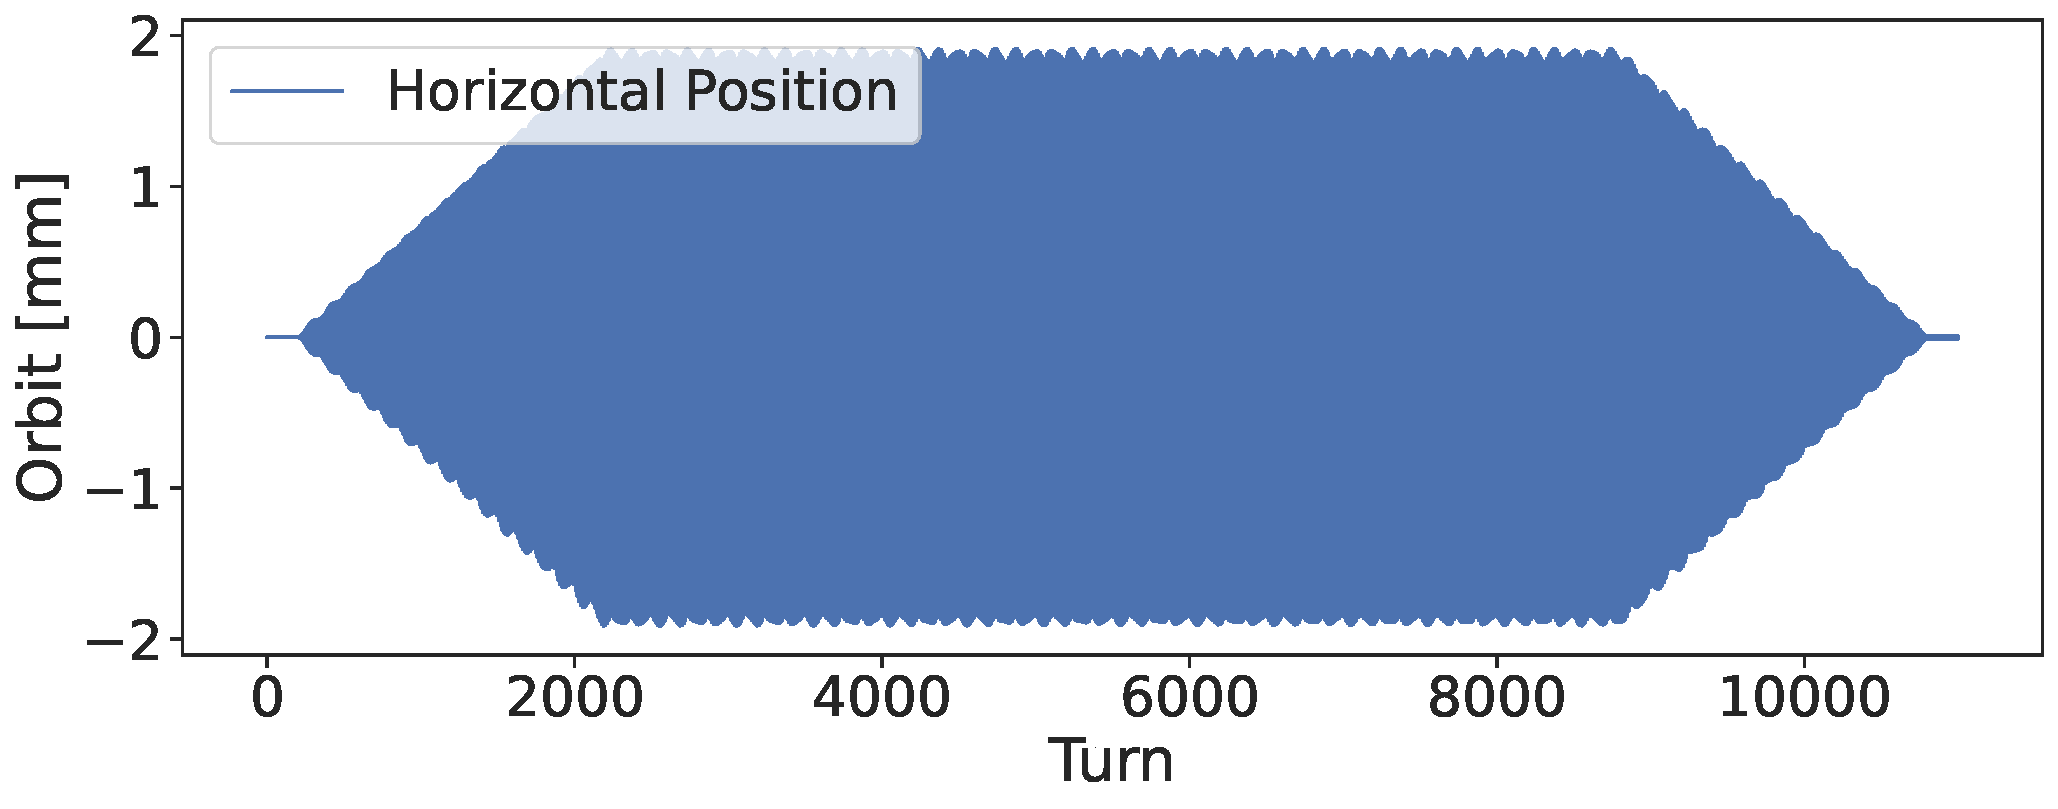
\includegraphics[width=0.85\textwidth]{./images/ac_dipole_tbt.pdf}
    \caption{Simulated turn-by-turn data with an AC-Dipole first ramping up then down.}
    \label{fig:ac_dipole}
\end{figure}

The AC-Dipole is set to oscillate at a frequency $Q_d$, different from the natural tune of the
machine $Q$ and thus introduces systematic effects that needs to be compensated during the optics
analysis. The transverse position of a particle, starting on the reference orbit, under the
influence of the AC-Dipole, at turn number $n$ and observation point $s$, is given
by~\cite{serrano_lhc_2010,tomas_normal_2002,white_direct_2013}:

\begin{equation}
z(s, n) = \frac{BL}{4\pi\rho\delta_z} \cdot \sqrt{\beta_z(s) \beta_{z,0}} \cdot \cos \left( 2 \pi Q_{d,z}n + \phi_z(s) + \phi_{z,0}\right),
\label{eq:ac_dipole}
\end{equation}

where $B$ is the amplitude of the oscillating magnetic field, $L$ the length of the AC-Dipole,
$B\rho$ the magnetic rigidity, $\delta$ the difference between $Q_d$ and $Q$, $\beta$ and $\beta_0$
the beta-function at the observed point and the AC-Dipole, $\phi$ and $\phi_0$ the phase advance at
the observed point and at the AC-Dipole.
